% ======================================================================
%  Chapter 6  --  Parametric Study
%
%  Split from the former combined chapter. Chapter 7 now carries the
%  calibration curves and the development length equation.
%
%  !! MISSING FROM YOUR .bib -- ADD BEFORE COMPILING !!
%     as3600ConcreteStructures2018   (AS 3600:2018)
%
%  CROSS-REFERENCES ASSUMED TO EXIST ELSEWHERE:
%     sec:closure  sec:failure  eq:capacity  eq:kbond  eq:slipfail
%     eq:slip  eq:solution  ch:tcd  chap:devlength
%
%  UNRESOLVED: \ref{} to Chapter~[X] in Sections 6.1.1
% ======================================================================

\chapter{Parametric Study of Factors Influencing Bond}
\label{chap:parametric}

The preceding chapters established the model and showed that it reproduces
the stress fields of two published analytical solutions. This chapter puts
it to work on the question it was built to answer: which properties of reinforced concrete affect anchorage, control its strength, its stiffness and the slip at which it
fails, and by how much.
 
Ten factors are examined, each varied about a common baseline while the
rest are held fixed. For every case the chapter reports the predicted
cracking load, the mean bond stress, the bond stiffness and the slip,
together with the two normalised stress components that identify how the
failure criterion is being satisfied. The outcome is a ranking of the
factors by influence, a decomposition of the concrete-strength effect into
its strength and stiffness parts, and an identification of the one
assumption in the formulation that is both unverified and consequential.
 
The findings established here are carried into
Chapter~\ref{chap:devlength}, which assembles them into calibration curves
and inverts those curves to give a development length expression.


% ======================================================================
\newpage
\section{Approach}
\label{sec:factorsapproach}

\subsection{Baseline specimen}

Every sweep changes one property at a time and holds the rest at the
baseline of Table~\ref{tab:factorbase}: a \SI{12}{\milli\metre} deformed bar
embedded \SI{150}{\milli\metre} into a \SI{150}{\milli\metre} diameter
cylinder of \SI{32}{\mega\pascal} concrete. This is the geometry of the
pull-out specimens used for comparison in Chapter~[X] and the case used for
the mesh study of Chapter~\ref{ch:tcd}.

\begin{table}[H]
\centering
\caption{Baseline specimen for the parametric study.}
\label{tab:factorbase}
\small
\begin{tabular*}{\linewidth}{@{\extracolsep{\fill}}llc@{}}
\hline
Property & Symbol & Value \\
\hline
Bar diameter                  & $d_b$          & \SI{12}{\milli\metre} \\
Embedment length              & $L$            & \SI{150}{\milli\metre} \\
Cylinder diameter             & $d_{cyl}$      & \SI{150}{\milli\metre} \\
Rib layer thickness           & $t_{rib}$      & \SI{0.5}{\milli\metre} \\
Concrete strength             & $f'_c$         & \SI{32}{\mega\pascal} \\
Concrete modulus              & $E_c$          & \SI{30100}{\mega\pascal} \\
Concrete Poisson's ratio      & $\nu_c$        & 0.20 \\
Steel modulus                 & $E_s$          & \SI{200}{\giga\pascal} \\
Steel yield stress            & $f_{sy}$       & \SI{550}{\mega\pascal} \\
Tensile and shear strength    & $f_t=f_v$      & $0.5\sqrt{f'_c}=\SI{2.83}{\mega\pascal}$ \\
Critical distance             & $l_{char}$     & \SI{20}{\milli\metre} \\
Item size                     & $l_{item}$     & \SI{2}{\milli\metre} \\
Loading configuration         & ---            & pull--push \\
\hline
\end{tabular*}
\end{table}

The concrete modulus follows Table 3.1.2 of
\textcite{as3600ConcreteStructures2018} and is therefore tied to $f'_c$
wherever the strength is varied. Section~\ref{sec:matstiff} breaks that tie
deliberately, and doing so resolves a discrepancy with the bond literature
that would otherwise be unexplained.

\subsection{Quantities reported}

Four outputs are reported for every case. The Mode~II cracking load
$F_{II}$ comes from the Area Method of Chapter~\ref{ch:tcd} through the
quadratic interaction index of \eqref{eq:capacity}. The mean bond stress
\begin{equation}
\label{eq:taubar}
\tau_u = \frac{F_u}{\pi d_b L}
\end{equation}
removes the trivial growth of capacity with bonded area and is the form in
which experimental bond correlations are reported. The bond stiffness
$k_s$ of \eqref{eq:kbond} and the slip $\delta_u$ of \eqref{eq:slipfail}
come from the same solved stress field at no additional cost. Both are \emph{initial} values: the formulation is linearly elastic, so \eqref{eq:slipfail} extrapolates the initial tangent
out to the cracking load. A measured bond--slip response softens
progressively well before its peak, so throughout this chapter $\delta_u$ is
a lower bound on measured slip and $k_s$ an upper bound on the
stiffness at peak load. Finally, the
two normalised stresses at the governing station,
\begin{equation}
\label{eq:normstress}
\hat\sigma = \frac{\bar\sigma_\theta}{f_t}\bigg|_{F_u},
\qquad
\hat\tau = \frac{\bar\tau_{rz}}{f_v}\bigg|_{F_u},
\qquad
\hat\sigma^2 + \hat\tau^2 = 1,
\end{equation}
record how the failure criterion is being satisfied, and so identify whether
a case is failing in hoop tension or in interfacial shear.

\subsection{Factors considered and the threshold for influence}

Ten factors are swept, in two groups: geometric (embedment length, bar
diameter at fixed $L$ and at fixed $L/d_b$, outer radius, rib layer
thickness) and material (concrete strength with $E_c$ tied, concrete modulus
with $f'_c$ fixed, shear-to-tensile strength ratio, Poisson's ratio, rib
layer modulus, steel modulus).
 
Influence is quantified throughout by the exponent $n$ of a power law
$F_{II} \propto x^{\,n}$ fitted across each swept range, because an exponent
is independent of the range chosen while a percentage change is not. A
factor is described as \emph{negligible} where $|n| < 0.05$, as
\emph{moderate} for $0.05 \le |n| \le 0.5$, and as \emph{dominant} above
that. 1

\subsection{Isolating a mechanism by removing it}

Two of the results below are obtained not by varying a property but by
breaking a link that is normally fixed. Concrete strength and modulus rise
together in any real concrete, so the sweep in Section~\ref{sec:matfc} can
only report their combined effect; Section~\ref{sec:matstiff} separates them
by holding the strength constant and varying the modulus alone, which is not
a physically realisable concrete but is a perfectly admissible numerical
experiment. The same logic identifies the cause of the non-monotonic cover
response in Section~\ref{sec:geomcover}. Where a mechanism is suspected, the
most direct test is to remove it and see whether the behaviour disappears.

\subsection{Factors outside the scope of the model}
\label{sec:outofscope}
Two factors that literature treats as essential are absent from the
model. Transverse confinement enters \textcite{orangunStrengthAnchoredBars}
through $K_{tr}$ and \textcite{408R03BondDevelopment} through the area and
spacing of ties, but no transverse steel is modelled here: the cylinder is
plain concrete with no spiral. The omission matters least at for large
cover, where the concrete ring confines the bar on its own, and most at
small cover where splitting governs, the same regime in which
Section~\ref{sec:geomcover} finds the averaging method least reliable.

Rib geometry, which \textcite{ngCustomisedRibPattern} exploit to shorten
development lengths for Grade~600 bars, is absent for the same kind of
reason: the bar modelled is plain, its interlock carried by a smeared rib
layer rather than by ribs of a given height, spacing and face angle. Only
that layer's thickness and modulus can be varied, and
Sections~\ref{sec:ribthick} and~\ref{sec:matminor} test both.

The two are not equally fundamental. A spiral is axisymmetric once smeared
into an equivalent radial stiffness, so confinement could be added to the
present formulation; discrete ribs are break the axial symmetry
it depends on, so rib geometry could not. Both are returned to in
Section~\ref{sec:paramconc}.


% ======================================================================
\newpage
\section{Geometric factors}
\label{sec:geomfactors}

% ----------------------------------------------------------------------
\subsection{Embedment length}
\label{sec:geomL}

Lengthening the anchorage raises the predicted cracking load, but only up to
a point. Table~\ref{tab:sweepL} shows the baseline bar embedded between
\SI{50}{} and \SI{300}{\milli\metre}: the load rises steeply to
\SI{100}{\milli\metre} and then stops, gaining \SI{1.1}{\percent} over the
remaining \SI{200}{\milli\metre}.

\begin{table}[H]
\centering
\caption{Effect of embedment length ($d_b = \SI{12}{\milli\metre}$).}
\label{tab:sweepL}
\small
\begin{tabular*}{\linewidth}{@{\extracolsep{\fill}}cccccccc@{}}
\hline
$L$ & $L/d_b$ & $F_{II}$ & $\tau_u$ & $k_s$ & $\delta_u$
    & $\hat\sigma$ & $\hat\tau$ \\
(mm) &        & (kN)     & (MPa)    & (kN/mm) & (mm) & & \\
\hline
50  & 4.17  & 9.310  & 4.939 & 537.0 & 0.01734 & 0.629 & 0.778 \\
75  & 6.25  & 12.054 & 4.263 & 621.9 & 0.01938 & 0.622 & 0.783 \\
100 & 8.33  & 12.597 & 3.341 & 630.7 & 0.01997 & 0.616 & 0.788 \\
125 & 10.42 & 12.668 & 2.688 & 631.3 & 0.02007 & 0.613 & 0.790 \\
150 & 12.50 & 12.688 & 2.244 & 631.2 & 0.02010 & 0.612 & 0.791 \\
200 & 16.67 & 12.709 & 1.686 & 631.2 & 0.02014 & 0.610 & 0.793 \\
250 & 20.83 & 12.722 & 1.350 & 631.1 & 0.02016 & 0.609 & 0.793 \\
300 & 25.00 & 12.731 & 1.126 & 631.1 & 0.02017 & 0.608 & 0.794 \\
\hline
\end{tabular*}
\end{table}

Three features of this table matter.

\paragraph{The mean bond stress falls, but the bond does not weaken.}
$\tau_u$ drops from \SI{4.94}{} to \SI{1.13}{\mega\pascal} across the
range, which follows from how the quantity is defined rather than from any
change in the concrete. The load itself has stopped growing:
Figure~\ref{fig:factorL} shows it flattening by about
\SI{100}{\milli\metre}, with a gain of only \SI{1.1}{\percent} as the
embedment then triples. Since $\tau_u = F_u/(\pi d_b L)$, a constant
load divided by a growing length must fall as $1/L$.

\paragraph{The stiffness levels off at the same embedment.}
By $L = \SI{125}{\milli\metre}$, it reaches
\SI{631}{\kilo\newton\per\milli\metre}, up from \SI{537}{}; it is then flat to within
\SI{0.03}{\percent}. This rules out an awkward objection. The averaging
disc has a radius of \SI{26.4}{\milli\metre} and sits at the loaded end, so
the failure criterion sees only the first \SI{27}{\milli\metre} of the bar,
and the capacity might stop growing simply because the criterion cannot
look further along. The stiffness answers that, because it is computed from
the energy stored over the \emph{whole} embedded length and uses nothing
from the criterion. Were the
flattening a blind spot, the capacity would level off while the stiffness
kept rising. Both flatten together, so load transfer is genuinely complete
by \SI{100}{\milli\metre}.

\paragraph{The slip at failure is constant.}
It holds at \SI{0.0201}{\milli\metre} for every embedment beyond
\SI{100}{\milli\metre}. This follows from the two results above, since
$\delta_u = F_u/k_s$ and both level off, but it is worth stating because it
is directly testable: first cracking is predicted at the same loaded-end
displacement however long the anchorage. The constancy holds along this
axis only: Section~\ref{sec:geomdb} shows $\delta_u$ falling as
$d_b^{-0.43}$ with bar diameter, so this is a stress criterion that
happens not to depend on length, not a slip criterion in disguise.

\begin{figure}[H]
\centering
\definecolor{mblue}{rgb}{0,0.4470,0.7410}
\pgfplotsset{
  bondaxis/.style={
    width=\linewidth, height=0.80\linewidth,
    xlabel={embedment length $L$ (mm)},
    xmin=25, xmax=325, xtick={50,100,150,200,250,300},
    grid=both,
    grid style={line width=0.2pt, draw=gray!20},
    major grid style={line width=0.3pt, draw=gray!40},
    tick label style={font=\small}, label style={font=\small},
    every axis plot/.append style={
      line width=0.9pt, mark=o, mark size=1.9pt, mark options={solid}},
  }
}
\begin{subfigure}[b]{0.48\linewidth}
\centering
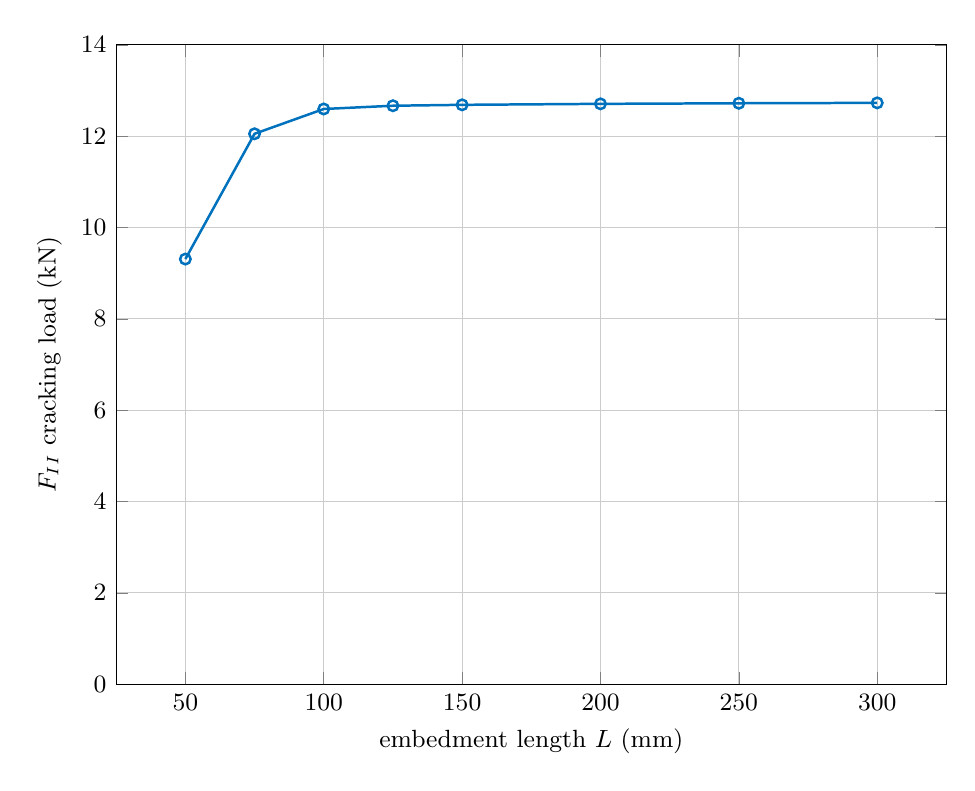
\begin{tikzpicture}
\begin{axis}[bondaxis,
  ylabel={$F_{II}$ cracking load (kN)},
  ymin=0, ymax=14, ytick={0,2,4,6,8,10,12,14}]
\addplot[mblue] coordinates {
  (50,9.3100) (75,12.0538) (100,12.5967) (125,12.6681)
  (150,12.6878) (200,12.7093) (250,12.7221) (300,12.7307)};
\end{axis}
\end{tikzpicture}
\caption{}
\label{fig:factorL-load}
\end{subfigure}
\hfill
\begin{subfigure}[b]{0.48\linewidth}
\centering
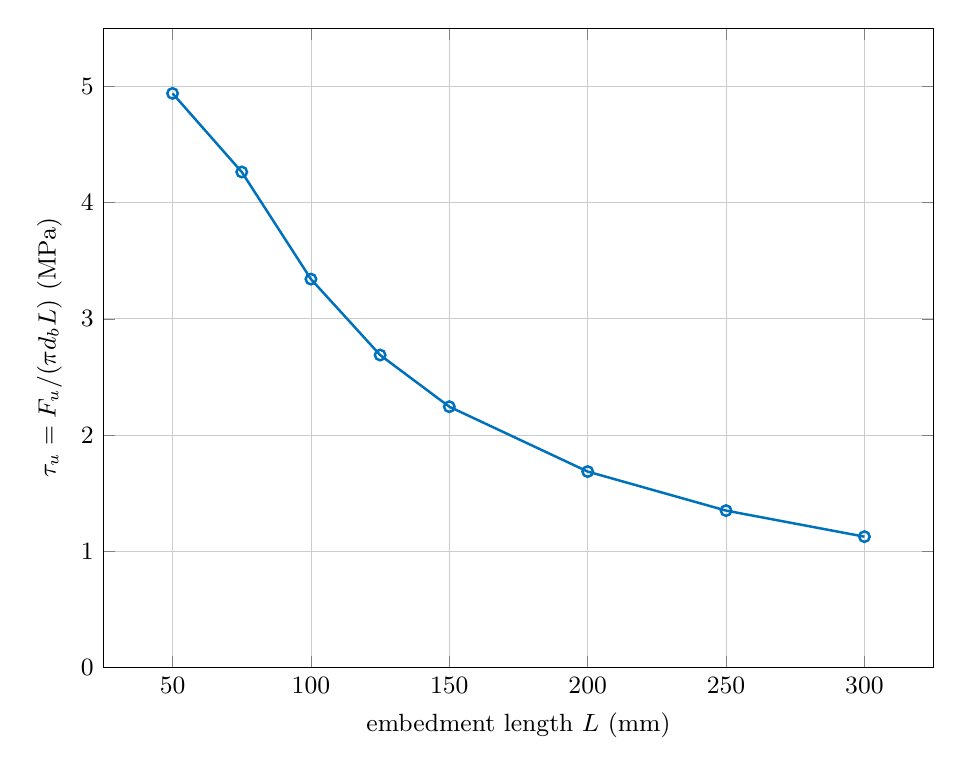
\begin{tikzpicture}
\begin{axis}[bondaxis,
  ylabel={$\tau_u = F_u/(\pi d_b L)$ (MPa)},
  ymin=0, ymax=5.5, ytick={0,1,2,3,4,5}]
\addplot[mblue] coordinates {
  (50,4.9391) (75,4.2632) (100,3.3414) (125,2.6883)
  (150,2.2437) (200,1.6856) (250,1.3499) (300,1.1256)};
\end{axis}
\end{tikzpicture}
\caption{}
\label{fig:factorL-tau}
\end{subfigure}
\caption{Effect of embedment length on the baseline specimen
         ($d_b = \SI{12}{\milli\metre}$, $f'_c = \SI{32}{\mega\pascal}$,
         $r_e = \SI{75}{\milli\metre}$). (a)~The predicted cracking load
         levels off by about \SI{100}{\milli\metre}, gaining only
         \SI{1.1}{\percent} over the remaining \SI{200}{\milli\metre}.
         (b)~The mean bond stress continues to fall as $1/L$, because a
         load that has stopped growing is being divided by a length that
         has not.}
\label{fig:factorL}
\end{figure}

% ----------------------------------------------------------------------
\subsection{Bar diameter}
\label{sec:geomdb}

Bar diameter is the most influential geometric factor.
Table~\ref{tab:sweepdb} varies it with the embedment held at the baseline,
and Table~\ref{tab:sweepdb2} repeats the sweep at a constant slenderness of
$L/d_b = 10$ so that bar size and slenderness can be separated.

\begin{table}[H]
\centering
\caption{Effect of bar diameter at fixed embedment length
         ($L = \SI{150}{\milli\metre}$).}
\label{tab:sweepdb}
\small
\begin{tabular*}{\linewidth}{@{\extracolsep{\fill}}cccccccc@{}}
\hline
$d_b$ & $L/d_b$ & $F_{II}$ & $\tau_u$ & $k_s$ & $\delta_u$
      & $\hat\sigma$ & $\hat\tau$ \\
(mm)  &        & (kN)      & (MPa)    & (kN/mm) & (mm) & & \\
\hline
8  & 18.75 & 8.826  & 2.341 & 365.0  & 0.02418 & 0.501 & 0.866 \\
10 & 15.00 & 10.760 & 2.283 & 494.1  & 0.02178 & 0.562 & 0.828 \\
12 & 12.50 & 12.688 & 2.244 & 631.2  & 0.02010 & 0.612 & 0.791 \\
16 & 9.38  & 16.443 & 2.181 & 924.0  & 0.01780 & 0.690 & 0.724 \\
20 & 7.50  & 19.983 & 2.120 & 1233.0 & 0.01621 & 0.747 & 0.665 \\
24 & 6.25  & 23.256 & 2.056 & 1550.1 & 0.01500 & 0.790 & 0.614 \\
\hline
\end{tabular*}
\end{table}

\begin{table}[H]
\centering
\caption{Effect of bar diameter at constant slenderness
         ($L/d_b = 10$, so the embedment varies with the bar).}
\label{tab:sweepdb2}
\small
\begin{tabular*}{\linewidth}{@{\extracolsep{\fill}}ccccccc@{}}
\hline
$d_b$ & $L$ & $F_{II}$ & $\tau_u$ & $k_s$ & $\delta_u$ & $\hat\sigma$ \\
(mm)  & (mm) & (kN)     & (MPa)    & (kN/mm) & (mm) & \\
\hline
8  & 80  & 8.770  & 4.362 & 364.9  & 0.02403 & 0.506 \\
10 & 100 & 10.722 & 3.413 & 494.0  & 0.02170 & 0.565 \\
12 & 120 & 12.662 & 2.799 & 631.3  & 0.02006 & 0.614 \\
16 & 160 & 16.456 & 2.046 & 923.9  & 0.01781 & 0.689 \\
20 & 200 & 20.067 & 1.597 & 1233.0 & 0.01627 & 0.745 \\
24 & 240 & 23.447 & 1.296 & 1550.6 & 0.01512 & 0.787 \\
\hline
\end{tabular*}
\end{table}

\paragraph{Cracking capacity grows almost in proportion to bar diameter.}
Fitting a power law to each table (Appendix~\ref{app:exponents}) gives
$F_{II} \propto d_b^{0.886}$ at fixed $L$ and $d_b^{0.898}$ at fixed
$L/d_b$, so
\begin{equation}
\label{eq:dbexp}
F_{II} \propto d_b^{0.89} ,
\end{equation}
close to direct proportionality (Figure~\ref{fig:factordb}). Capacity is
not proportional to the bonded area $\pi d_b L$: at constant slenderness
that area grows ninefold while the capacity grows only \num{2.67}-fold.
Load transfer is confined to a zone near the loaded end that does not
lengthen with the bar (Section~\ref{sec:geomL}), so most of the added
interface carries almost nothing.

Demand grows faster. The yield force $A_s f_{sy}$ goes as $d_b^{2}$
against the $d_b^{0.89}$ of \eqref{eq:dbexp}, so doubling the bar
multiplies capacity by \num{1.85} and demand by four. This is the
chapter's most consequential result, and the mechanical reason anchoring
large high-grade bars is the binding constraint identified by
\textcite{ngChangesAustralianStandards}.

\paragraph{The failure mode shifts with bar size.}
Squaring the last two columns of Table~\ref{tab:sweepdb} gives each
mechanism's share of the failure criterion, the two summing to one. At
$d_b = \SI{8}{\milli\metre}$ the split is \SI{75}{\percent} shear to
\SI{25}{\percent} hoop; by \SI{24}{\milli\metre} it has reversed to
\SI{38}{} and \SI{62}{\percent}, crossing near \SI{17}{\milli\metre}. Shear
is a pull-out failure and hoop tension a splitting failure, so the model
predicts small bars pulling out and large bars splitting, the transition
reported by \textcite{liTensileBondAnchorage2012} and one it was not
fitted to reproduce.

\paragraph{Stiffness grows faster than strength.}
The bond stiffness rises as $k_s \propto d_b^{1.32}$, faster than the
capacity, so the slip at failure falls as the difference of the exponents,
$\delta_u \propto d_b^{-0.43}$. Against a free bar of the same size the
anchorage is stiffer by a falling margin, \num{5.45} times at
\SI{8}{\milli\metre} against \num{2.57} at \SI{24}{\milli\metre}, because
only the loaded end is ever stretched and that region is relatively
shorter for a small bar.

\begin{figure}[H]
\centering
\definecolor{mblue}{rgb}{0,0.4470,0.7410}
\pgfplotsset{
  dbaxis/.style={
    width=\linewidth, height=0.80\linewidth,
    xlabel={bar diameter $d_b$ (mm)},
    xmin=0, xmax=26, xtick={0,4,8,12,16,20,24},
    grid=both,
    grid style={line width=0.2pt, draw=gray!20},
    major grid style={line width=0.3pt, draw=gray!40},
    tick label style={font=\small}, label style={font=\small},
    every axis plot/.append style={
      line width=0.9pt, mark=o, mark size=1.9pt, mark options={solid}},
  }
}
\begin{subfigure}[b]{0.48\linewidth}
\centering
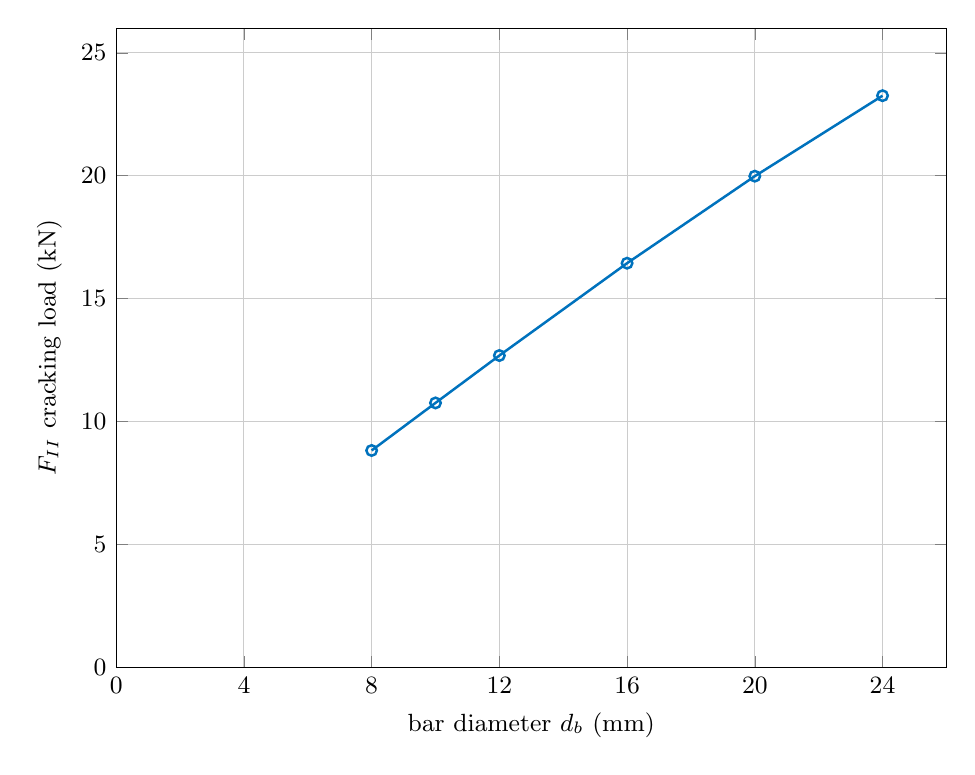
\begin{tikzpicture}
\begin{axis}[dbaxis,
  ylabel={$F_{II}$ cracking load (kN)},
  ymin=0, ymax=26, ytick={0,5,10,15,20,25}]
\addplot[mblue] coordinates {
  (8,8.8256) (10,10.7601) (12,12.6878)
  (16,16.4431) (20,19.9828) (24,23.2561)};
\end{axis}
\end{tikzpicture}
\caption{}
\label{fig:factordb-load}
\end{subfigure}
\hfill
\begin{subfigure}[b]{0.48\linewidth}
\centering
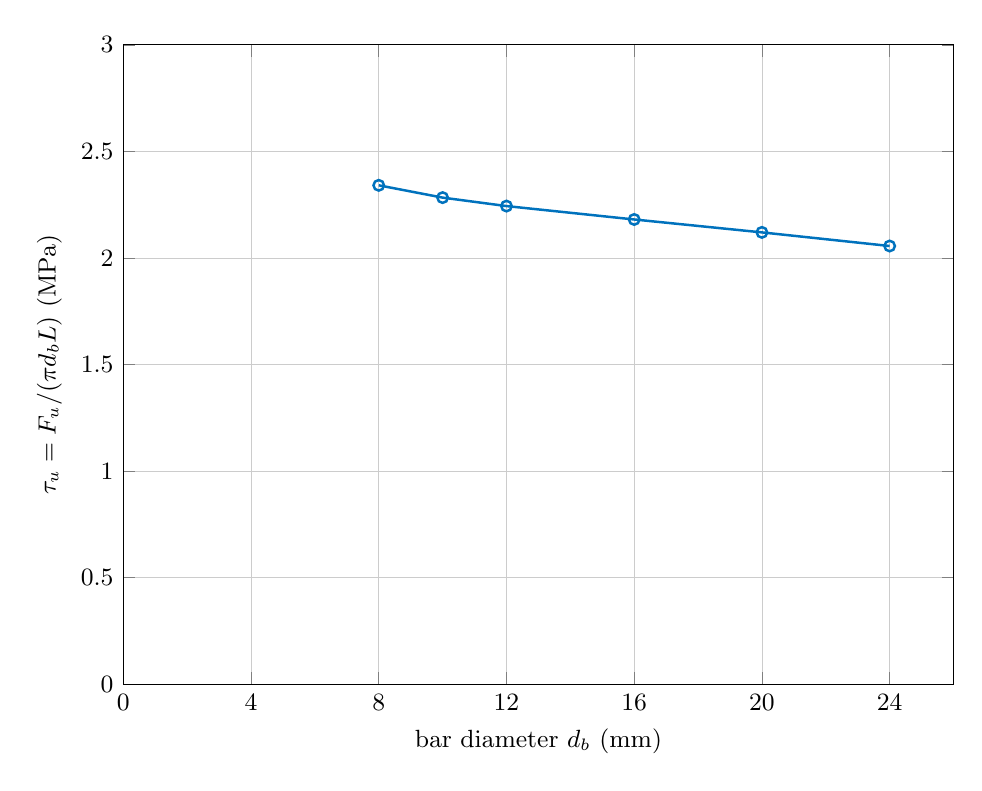
\begin{tikzpicture}
\begin{axis}[dbaxis,
  ylabel={$\tau_u = F_u/(\pi d_b L)$ (MPa)},
  ymin=0, ymax=3, ytick={0,0.5,1,1.5,2,2.5,3}]
\addplot[mblue] coordinates {
  (8,2.3411) (10,2.2834) (12,2.2437)
  (16,2.1808) (20,2.1202) (24,2.0563)};
\end{axis}
\end{tikzpicture}
\caption{}
\label{fig:factordb-tau}
\end{subfigure}
\caption{Effect of bar diameter at fixed embedment
         ($L = \SI{150}{\milli\metre}$, $f'_c = \SI{32}{\mega\pascal}$,
         $r_e = \SI{75}{\milli\metre}$). (a)~The cracking load rises almost
         in proportion to the diameter, following $d_b^{0.89}$.
         (b)~The mean bond stress is nearly constant, falling only
         \SI{12}{\percent} over a threefold increase in bar size, which is
         the same result seen another way.}
\label{fig:factordb}
\end{figure}

% ----------------------------------------------------------------------
\subsection{Cover ratio}
\label{sec:geomcover}

Cover is the dominant geometric variable in every empirical bond model: it
appears as $c/d_b$ in \textcite{orangunStrengthAnchoredBars}, as
$(c+0.5d_b)$ in \textcite{SpliceStrengthConventional2000}, and
\textcite{hadiBondHighStrength2008} isolates it by casting the same bars in
two cylinder sizes. Here it enters through the outer radius $r_e$ and is
reported as
\begin{equation}
\label{eq:coverratio}
\frac{c}{d_b} = \frac{r_e - d_b/2}{d_b}.
\end{equation}

\begin{table}[H]
\centering
\caption{Effect of concrete cover ($d_b = \SI{12}{\milli\metre}$,
         $L = \SI{150}{\milli\metre}$). The first two rows are not
         comparable with the rest; see the text.}
\label{tab:sweepcover}
\small
\begin{tabular*}{\linewidth}{@{\extracolsep{\fill}}cccccccc@{}}
\hline
$r_e$ & $c/d_b$ & radial items & $F_{II}$ & $\tau_u$ & $k_s$ & $\delta_u$
      & $\hat\sigma$ \\
(mm)  &         & (of 14 needed) & (kN)   & (MPa)    & (kN/mm) & (mm) & \\
\hline
25  & 1.58 & 9$^{\dagger}$  & 10.087 & 1.784 & 826.0 & 0.01221 & 0.252 \\
30  & 2.00 & 12$^{\dagger}$ & 11.393 & 2.015 & 808.4 & 0.01409 & 0.348 \\
40  & 2.83 & 17 & 11.079 & 1.959 & 761.9 & 0.01454 & 0.489 \\
50  & 3.67 & 22 & 11.282 & 1.995 & 717.4 & 0.01573 & 0.548 \\
60  & 4.50 & 27 & 11.768 & 2.081 & 678.9 & 0.01734 & 0.582 \\
75  & 5.75 & 34 & 12.688 & 2.244 & 631.2 & 0.02010 & 0.612 \\
90  & 7.00 & 42 & 13.696 & 2.422 & 593.0 & 0.02310 & 0.631 \\
110 & 8.67 & 52 & 15.091 & 2.669 & 552.2 & 0.02733 & 0.648 \\
\hline
\multicolumn{8}{@{}p{0.95\linewidth}@{}}{\raggedright $^{\dagger}$~The
   averaging disc of radius $R_{avg} = \SI{26.4}{\milli\metre}$ does not fit
   inside the concrete and is clipped at the outer face, so these two cases
   average over less material than the rest and are not directly
   comparable.} \\
\hline
\end{tabular*}
\end{table}

\paragraph{Two points must be set aside.}
The load in Table~\ref{tab:sweepcover} does not rise steadily: it climbs
from \SI{10.09}{} to \SI{11.39}{\kilo\newton} between
$r_e = \SI{25}{}$ and \SI{30}{\milli\metre}, then \emph{falls} to
\SI{11.08}{\kilo\newton} at \SI{40}{\milli\metre}. Since the only thing
changing is the amount of concrete, that dip needs explaining, and the
cause turns out to be numerical rather than physical.

The Area Method averages the stress over a half-disc of radius
\SI{26.4}{\milli\metre} centred on the bar. In the two smallest specimens
that disc does not fit inside the concrete, so it is cut short at the outer
face and the criterion averages over a smaller and more highly stressed
region than elsewhere. The hoop share confirms it: \num{0.25} in the first
row against \num{0.49} in the first uncut row, so those two cases are
evaluating a different stress state, not simply a smaller one. They are
shown as open markers in Figure~\ref{fig:factorcov}, and the solver now
warns whenever the disc is cut.

Setting them aside, the remaining six points rise steadily and give
\begin{equation}
\label{eq:coverfit}
F_{II} \propto \left(\frac{c}{d_b}\right)^{0.281},
\qquad R^2 = 0.943 ,
\end{equation}
a \SI{36}{\percent} gain as the cover ratio rises from \num{2.83} to
\num{8.67}. Fitting all eight would have given \num{0.199} with
$R^2 = 0.857$: the two cut cases pull the exponent down by nearly a third.

\paragraph{The cover effect is weaker than measurements show.}
An exponent of \num{0.28} is modest beside the cover terms of
\textcite{orangunStrengthAnchoredBars}, and the reason is built into the
method. Concrete more than \SI{26.4}{\milli\metre} from the bar lies outside the
averaging disc, so it is never sampled directly; it reaches the stresses
that decide failure only indirectly, by stiffening the surrounding ring
and redistributing the field. That indirect route is the weaker of the
two, which is why the model understates the benefit of cover whenever the
cover exceeds the disc radius, here $c/d_b \gtrsim 2.2$.

\paragraph{Cover buys strength but costs stiffness.}
Across the six admissible points the capacity rises by \SI{36}{\percent}
while the stiffness \emph{falls} by \SI{28}{\percent} and the slip at
failure almost doubles. A thicker ring of concrete carries lower stress and
spreads the load transfer over a longer part of the bar, so more of the bar
stretches and the loaded end moves further. In design terms, extra cover
improves resistance to splitting but does nothing for stiffness in
service, and slightly worsens it. The hoop share rises from \num{0.49} to
\num{0.65} over the same range, so more cover also pushes the predicted
failure towards splitting.

\begin{figure}[H]
\centering
\definecolor{mblue}{rgb}{0,0.4470,0.7410}
\definecolor{mgrey}{rgb}{0.60,0.60,0.60}
\pgfplotsset{
  covaxis/.style={
    width=\linewidth, height=0.68\linewidth,
    xlabel={cover ratio $c/d_b$},
    xmin=0, xmax=9.5, xtick={0,2,4,6,8},
    grid=both,
    grid style={line width=0.2pt, draw=gray!20},
    major grid style={line width=0.3pt, draw=gray!40},
    tick label style={font=\small}, label style={font=\small},
    legend style={font=\scriptsize, at={(0.97,0.03)}, anchor=south east,
                  draw=none, fill=none, row sep=-2pt},
  }
}
\begin{subfigure}[b]{0.48\linewidth}
\centering
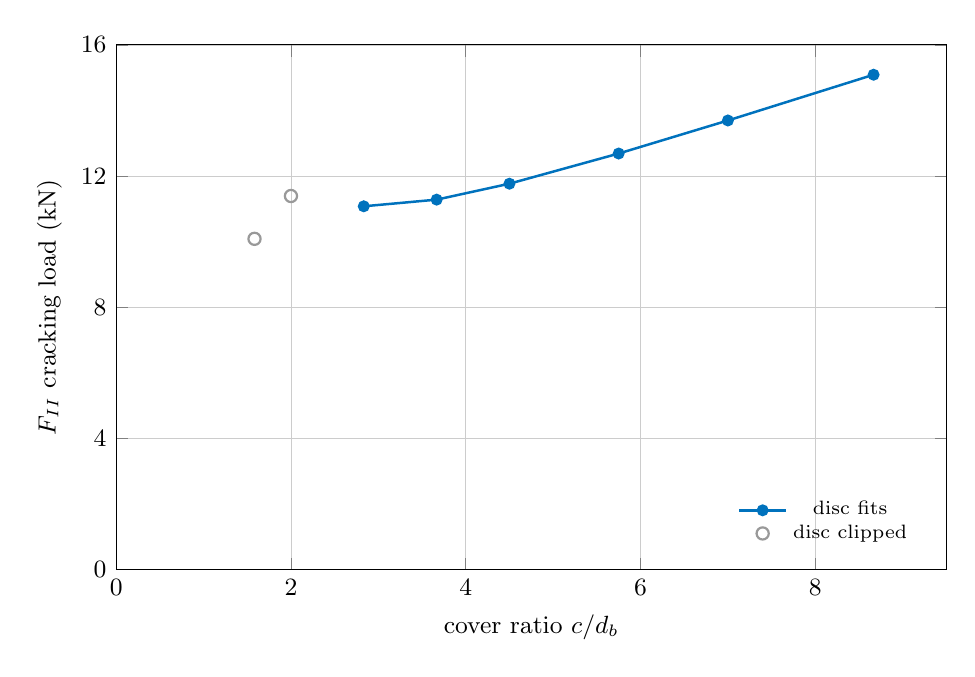
\begin{tikzpicture}
\begin{axis}[covaxis,
  ylabel={$F_{II}$ cracking load (kN)},
  ymin=0, ymax=16, ytick={0,4,8,12,16}]
\addplot[mblue, line width=0.9pt, mark=*, mark size=1.7pt]
  coordinates {(2.833,11.079) (3.667,11.282) (4.500,11.768)
               (5.750,12.688) (7.000,13.696) (8.667,15.091)};
\addlegendentry{disc fits}
\addplot[mgrey, only marks, mark=o, mark size=2.2pt, line width=0.8pt]
  coordinates {(1.583,10.087) (2.000,11.393)};
\addlegendentry{disc clipped}
\end{axis}
\end{tikzpicture}
\caption{}
\label{fig:factorcov-load}
\end{subfigure}
\hfill
\begin{subfigure}[b]{0.48\linewidth}
\centering
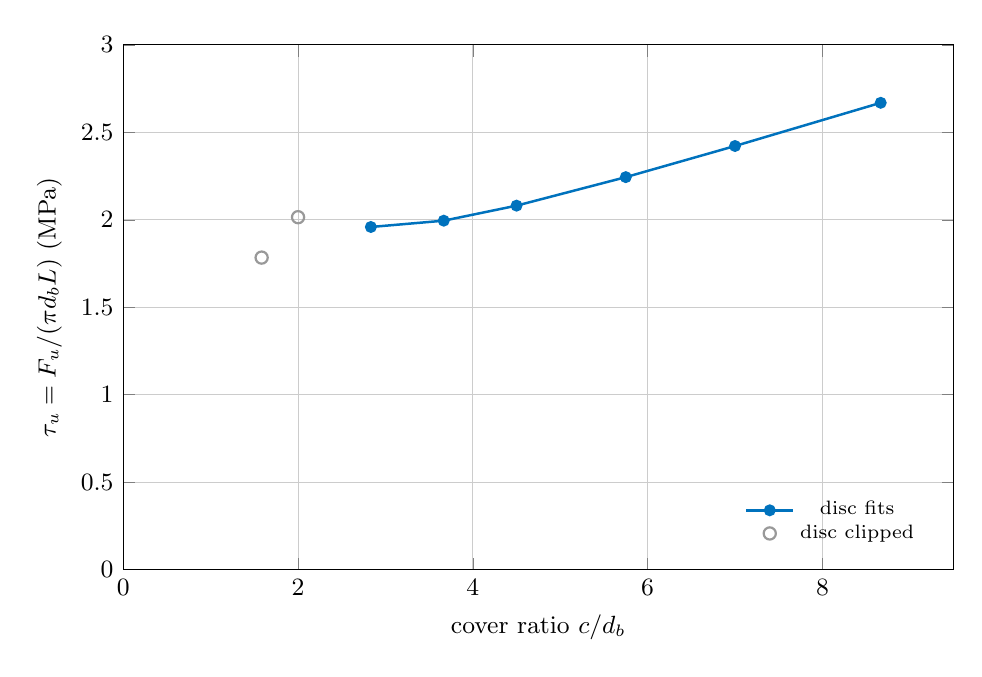
\begin{tikzpicture}
\begin{axis}[covaxis,
  ylabel={$\tau_u = F_u/(\pi d_b L)$ (MPa)},
  ymin=0, ymax=3, ytick={0,0.5,1,1.5,2,2.5,3}]
\addplot[mblue, line width=0.9pt, mark=*, mark size=1.7pt]
  coordinates {(2.833,1.959) (3.667,1.995) (4.500,2.081)
               (5.750,2.244) (7.000,2.422) (8.667,2.669)};
\addlegendentry{disc fits}
\addplot[mgrey, only marks, mark=o, mark size=2.2pt, line width=0.8pt]
  coordinates {(1.583,1.784) (2.000,2.015)};
\addlegendentry{disc clipped}
\end{axis}
\end{tikzpicture}
\caption{}
\label{fig:factorcov-tau}
\end{subfigure}
\caption{Effect of concrete cover ($d_b = \SI{12}{\milli\metre}$,
         $L = \SI{150}{\milli\metre}$, $f'_c = \SI{32}{\mega\pascal}$) on
         (a)~the cracking load and (b)~the mean bond stress. The two open
         markers are the cases in which the averaging disc does not fit
         inside the concrete and is cut short at the outer face; they are
         excluded from the fit of \eqref{eq:coverfit}. The remaining six
         points rise steadily.}
\label{fig:factorcov}
\end{figure}

% ----------------------------------------------------------------------
\subsection{Rib layer thickness}
\label{sec:ribthick}

The rib layer is the least physically grounded part of the idealisation. It
stands in for the mechanical interlock between the lugs and the surrounding
concrete, and in the implementation it is an annulus assigned the same
moduli as the concrete. Rib geometry measurably changes real bond
behaviour (Section~\ref{sec:outofscope}), so a layer that smears it away
needs its sensitivity established rather than assumed.

\begin{table}[H]
\centering
\caption{Sensitivity to the assumed rib layer thickness.}
\label{tab:sweeprib}
\small
\begin{tabular*}{\linewidth}{@{\extracolsep{\fill}}ccccc@{}}
\hline
$t_{rib}$ (mm) & $F_{II}$ (kN) & $\tau_u$ (MPa) & $k_s$ (kN/mm)
               & $\delta_u$ (mm) \\
\hline
0.25 & 12.691 & 2.244 & 631.5 & 0.02010 \\
0.50 & 12.688 & 2.244 & 631.2 & 0.02010 \\
0.75 & 12.685 & 2.243 & 631.0 & 0.02010 \\
1.00 & 12.680 & 2.242 & 630.7 & 0.02010 \\
1.50 & 12.676 & 2.242 & 630.2 & 0.02012 \\
2.00 & 12.672 & 2.241 & 629.6 & 0.02013 \\
\hline
\end{tabular*}
\end{table}

An eightfold change in the assumed thickness moves the capacity by
\SI{0.15}{\percent} and the stiffness by \SI{0.30}{\percent}. The rib layer
is a harmless numerical device: it supplies
the kinematic continuity the three-layer formulation requires without
influencing the answer. Whatever limitations the model has, they do not
arise from this parameter.


% ======================================================================
\section{Material factors}
\label{sec:matfactors}

% ----------------------------------------------------------------------
\subsection{Concrete strength}
\label{sec:matfc}
 
Concrete strength enters the model twice: through the strengths
$f_t = f_v = 0.5\sqrt{f'_c}$ that normalise the interaction index, and
through the modulus $E_c$ that determines how stress is distributed in the
first place. Table~\ref{tab:sweepfc} varies both together, as they vary
together in a real concrete.
 
\begin{table}[H]
\centering
\caption{Effect of concrete strength, with $E_c$ following
         \textcite{as3600ConcreteStructures2018} Table 3.1.2.}
\label{tab:sweepfc}
\small
\begin{tabular*}{\linewidth}{@{\extracolsep{\fill}}cccccc@{}}
\hline
$f'_c$ & $E_c$ & $F_{II}$ & $\tau_u$ & $k_s$ & $\delta_u$ \\
(MPa)  & (MPa) & (kN)      & (MPa)    & (kN/mm) & (mm) \\
\hline
20 & 24000 & 10.770 & 1.905 & 577.7 & 0.01864 \\
25 & 26700 & 11.642 & 2.059 & 602.5 & 0.01932 \\
32 & 30100 & 12.688 & 2.244 & 631.2 & 0.02010 \\
40 & 32800 & 13.815 & 2.443 & 652.3 & 0.02118 \\
50 & 34800 & 15.170 & 2.683 & 667.1 & 0.02274 \\
65 & 37400 & 16.925 & 2.993 & 685.4 & 0.02469 \\
80 & 39600 & 18.459 & 3.264 & 700.1 & 0.02637 \\
\hline
\end{tabular*}
\end{table}
 
A power law fitted across the range gives
\begin{equation}
\label{eq:fcexp}
\tau_u \propto (f'_c)^{0.390}, \qquad R^2 = 0.998 .
\end{equation}
 
This sits between the two values the literature offers. If capacity were
controlled by strength alone it would follow $f_t \propto \sqrt{f'_c}$ and
the exponent would be \num{0.50}; the descriptive equations of
\textcite{orangunStrengthAnchoredBars} normalise by $\sqrt{f'_c}$ on exactly
that reasoning. Against this, \textcite{SpliceStrengthConventional2000}
found that splice strength without confining reinforcement is better
characterised by $(f'_c)^{1/4}$, and
\textcite{408R03BondDevelopment} adopted the quarter power.
 
\textcite{harajliComparisonBondStrength2004} reconciles the two by showing
that the appropriate exponent depends on the development length: the quarter
power collapses normal- and high-strength data for $L/d_b \gtrsim 17$--$20$
while under-representing the effect of $f'_c$ at shorter lengths. The
present baseline, at $L/d_b = 12.5$, lies below that threshold, so an
exponent above \num{0.25} is what Harajli's finding would lead one to
expect. Section~\ref{sec:matstiff} accounts for the remainder of the gap
below \num{0.50}.
 
Figure~\ref{fig:factorfc} shows the trend, and three further points follow
from it.
 
\emph{The return on extra strength diminishes.} Going from \SI{20}{} to
\SI{25}{\mega\pascal} buys \SI{0.174}{\kilo\newton} of capacity for each
megapascal added, but going from \SI{65}{} to \SI{80}{\mega\pascal} buys
only \SI{0.102}{\kilo\newton}, a fall of \SI{41}{\percent}. Any exponent
below one behaves this way, and it is the gentle flattening of the curves
in Figure~\ref{fig:factorfc}.

\emph{The exponent is not quite constant.} Fitting between each pair of
successive points, rather than across the whole range at once, gives a
value that climbs steadily from \num{0.349} at the bottom to \num{0.418}
at the top. Equation~\eqref{eq:fcexp} is therefore a good approximation
over the range tested rather than an exact description, and
Section~\ref{sec:matstiff} identifies the cause.

\emph{Stiffness benefits far less than strength.} The bond stiffness
follows $k_s \propto (f'_c)^{0.137}$, so quadrupling the concrete strength
raises the capacity by \SI{71}{\percent} but the stiffness by only
\SI{21}{\percent}. The slip at failure follows from those two, since
$\delta_u = F_u/k_s$, and grows by \SI{41}{\percent}: a stronger concrete
carries more load without becoming proportionally stiffer, so it stretches
further before it cracks.

\begin{figure}[H]
\centering
\definecolor{mblue}{rgb}{0,0.4470,0.7410}
\pgfplotsset{
  fcaxis/.style={
    width=\linewidth, height=0.68\linewidth,
    xlabel={concrete strength $f'_c$ (MPa)},
    xmin=0, xmax=88, xtick={0,20,40,60,80},
    grid=both,
    grid style={line width=0.2pt, draw=gray!20},
    major grid style={line width=0.3pt, draw=gray!40},
    tick label style={font=\small}, label style={font=\small},
    every axis plot/.append style={
      line width=0.9pt, mark=o, mark size=1.8pt, mark options={solid}},
  }
}
\begin{subfigure}[b]{0.48\linewidth}
\centering
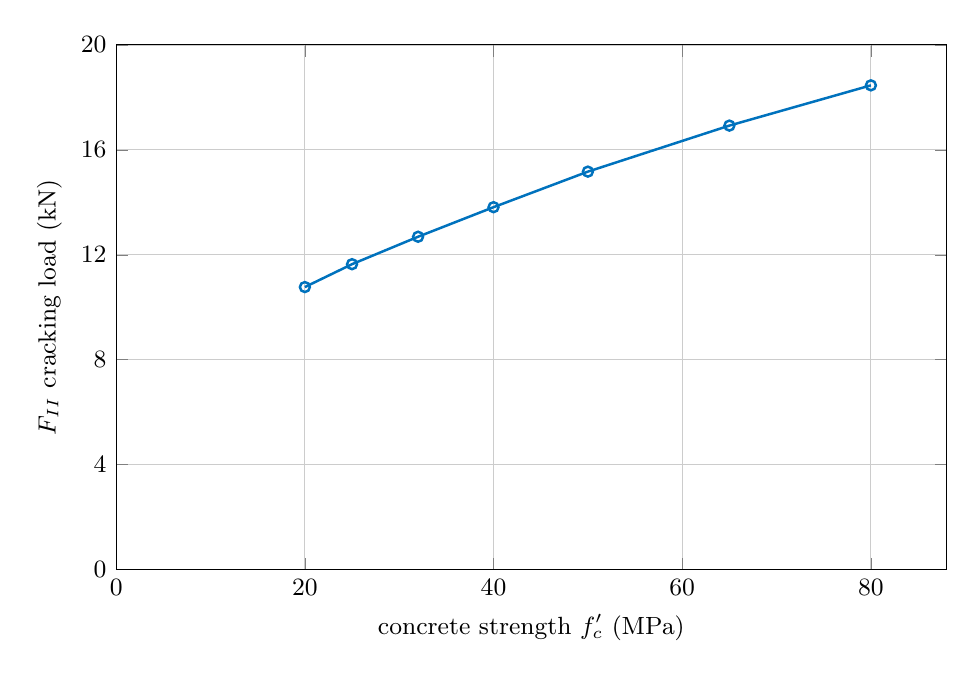
\begin{tikzpicture}
\begin{axis}[fcaxis,
  ylabel={$F_{II}$ cracking load (kN)},
  ymin=0, ymax=20, ytick={0,4,8,12,16,20}]
\addplot[mblue] coordinates {
  (20,10.770) (25,11.642) (32,12.688) (40,13.815)
  (50,15.170) (65,16.925) (80,18.459)};
\end{axis}
\end{tikzpicture}
\caption{}
\label{fig:factorfc-load}
\end{subfigure}
\hfill
\begin{subfigure}[b]{0.48\linewidth}
\centering
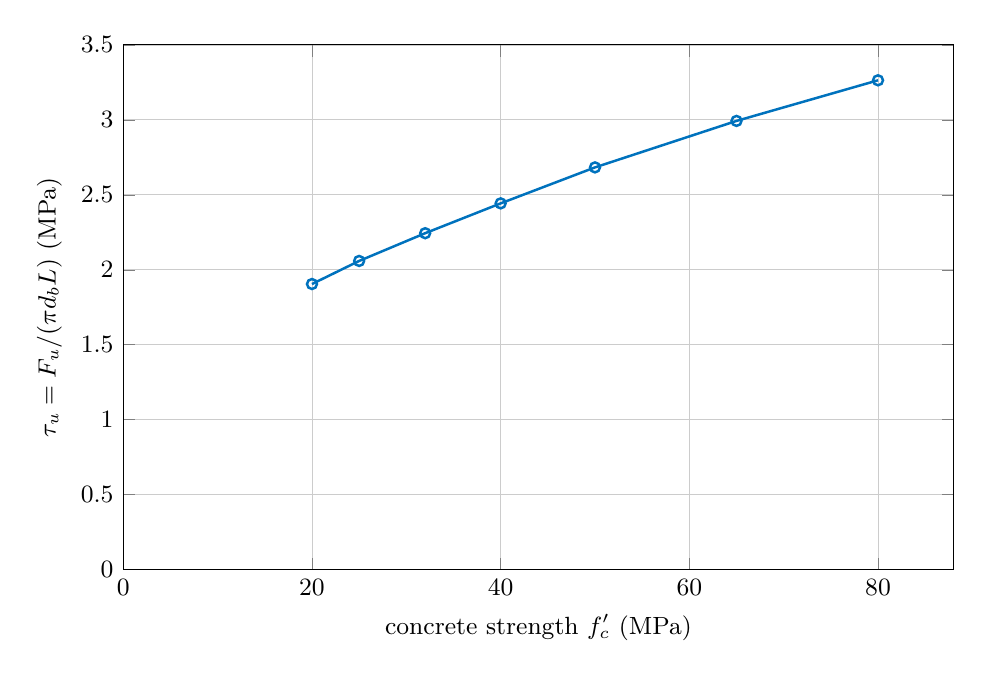
\begin{tikzpicture}
\begin{axis}[fcaxis,
  ylabel={$\tau_u = F_u/(\pi d_b L)$ (MPa)},
  ymin=0, ymax=3.5, ytick={0,0.5,1,1.5,2,2.5,3,3.5}]
\addplot[mblue] coordinates {
  (20,1.905) (25,2.059) (32,2.244) (40,2.443)
  (50,2.683) (65,2.993) (80,3.264)};
\end{axis}
\end{tikzpicture}
\caption{}
\label{fig:factorfc-tau}
\end{subfigure}
\caption{Effect of concrete strength, with $E_c$ following
         \textcite{as3600ConcreteStructures2018} Table 3.1.2
         ($d_b = \SI{12}{\milli\metre}$, $L = \SI{150}{\milli\metre}$,
         $r_e = \SI{75}{\milli\metre}$). (a)~The predicted cracking load
         and (b)~the mean bond stress, both rising as $(f'_c)^{0.390}$ and
         flattening gently as the strength increases. Because $d_b$ and
         $L$ are fixed throughout this sweep the two differ only by the
         constant bonded area.}
\label{fig:factorfc}
\end{figure}

% ----------------------------------------------------------------------
\newpage
\subsection{Concrete stiffness}
\label{sec:matstiff}

Because the elastic modulus $E_c$ and the strength $f'_c$ were tied in the
previous sweep their separate contributions cannot be read from it.
Table~\ref{tab:sweepEc} breaks the tie by varying the modulus at constant
strength, so that $f_t$ and $f_v$ are fixed and only the stress
distribution changes.

\begin{table}[H]
\centering
\caption{Effect of concrete modulus at constant strength
         ($f'_c = \SI{32}{\mega\pascal}$, so $f_t = f_v$ unchanged).}
\label{tab:sweepEc}
\small
\begin{tabular*}{\linewidth}{@{\extracolsep{\fill}}ccccc@{}}
\hline
$E_c$ (MPa) & $F_{II}$ (kN) & $\tau_u$ (MPa) & $k_s$ (kN/mm) & $\delta_u$ (mm) \\
\hline
24000 & 13.623 & 2.409 & 577.7 & 0.02358 \\
27000 & 13.125 & 2.321 & 605.2 & 0.02169 \\
30100 & 12.688 & 2.244 & 631.2 & 0.02010 \\
33000 & 12.334 & 2.181 & 653.8 & 0.01886 \\
36000 & 12.012 & 2.124 & 675.7 & 0.01778 \\
40000 & 11.640 & 2.058 & 702.7 & 0.01656 \\
\hline
\end{tabular*}
\end{table}

The capacity \emph{falls} as the modulus rises, following
$\tau_u \propto E_c^{-0.308}$. The reason is that a stiffer ring of
concrete takes up more of the load close to the bar, which is exactly
where the averaging disc looks. At a given applied force the stresses
there are therefore higher, so the failure criterion is satisfied at a
lower load. The \emph{bond} stiffness itself rises, as it must, following
$k_s \propto E_c^{0.384}$.

Section~\ref{sec:matfc} found the capacity rising as $(f'_c)^{0.390}$, and
the elastic modulus is why that exponent is not \num{0.500}. Strength
enters the criterion as $f_t = f_v = 0.5\sqrt{f'_c}$, so on its own it would make the
capacity rise as the square root of $f'_c$. But
a stronger concrete is also a stiffer one, and stiffness works the other
way, as this sweep shows. The two partly cancel, costing roughly a fifth
of that half. The quarter power of
\textcite{SpliceStrengthConventional2000} is on this reading not an
anomaly but a consequence of the two rising together.
Appendix~\ref{app:exponents} sets out the arithmetic.

\begin{figure}[H]
\centering
\definecolor{mblue}{rgb}{0,0.4470,0.7410}
\pgfplotsset{
  ecaxis/.style={
    width=\linewidth, height=0.68\linewidth,
    xlabel={concrete modulus $E_c$ (GPa)},
    xmin=21, xmax=43, xtick={24,28,32,36,40},
    grid=both,
    grid style={line width=0.2pt, draw=gray!20},
    major grid style={line width=0.3pt, draw=gray!40},
    tick label style={font=\small}, label style={font=\small},
    every axis plot/.append style={
      line width=0.9pt, mark=o, mark size=1.8pt, mark options={solid}},
  }
}
\begin{subfigure}[b]{0.48\linewidth}
\centering
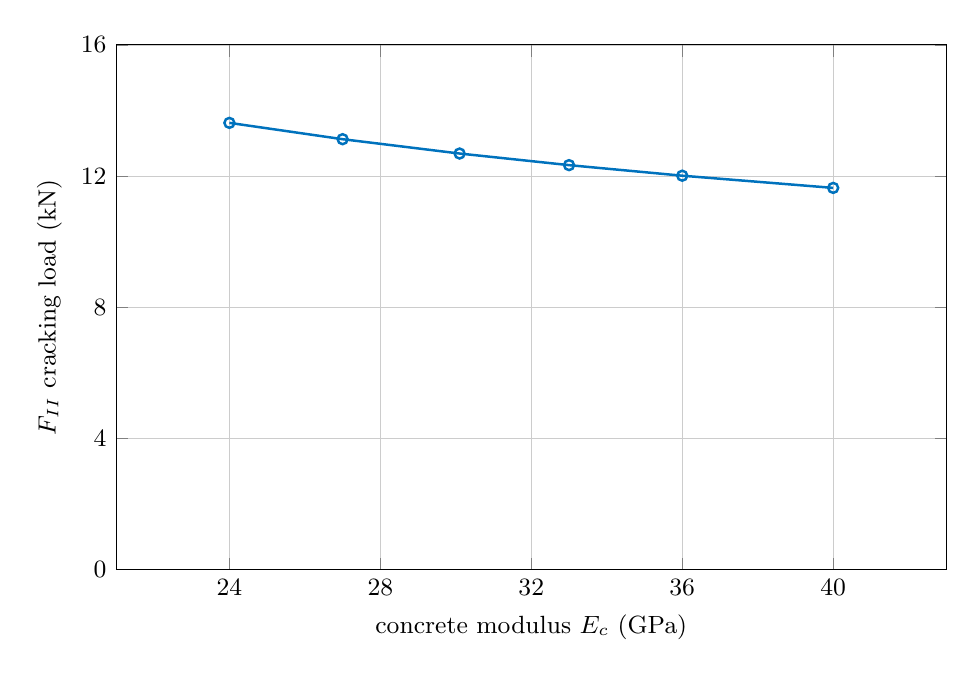
\begin{tikzpicture}
\begin{axis}[ecaxis,
  ylabel={$F_{II}$ cracking load (kN)},
  ymin=0, ymax=16, ytick={0,4,8,12,16}]
\addplot[mblue] coordinates {
  (24.0,13.623) (27.0,13.125) (30.1,12.688)
  (33.0,12.334) (36.0,12.012) (40.0,11.640)};
\end{axis}
\end{tikzpicture}
\caption{}
\label{fig:factorEc-load}
\end{subfigure}
\hfill
\begin{subfigure}[b]{0.48\linewidth}
\centering
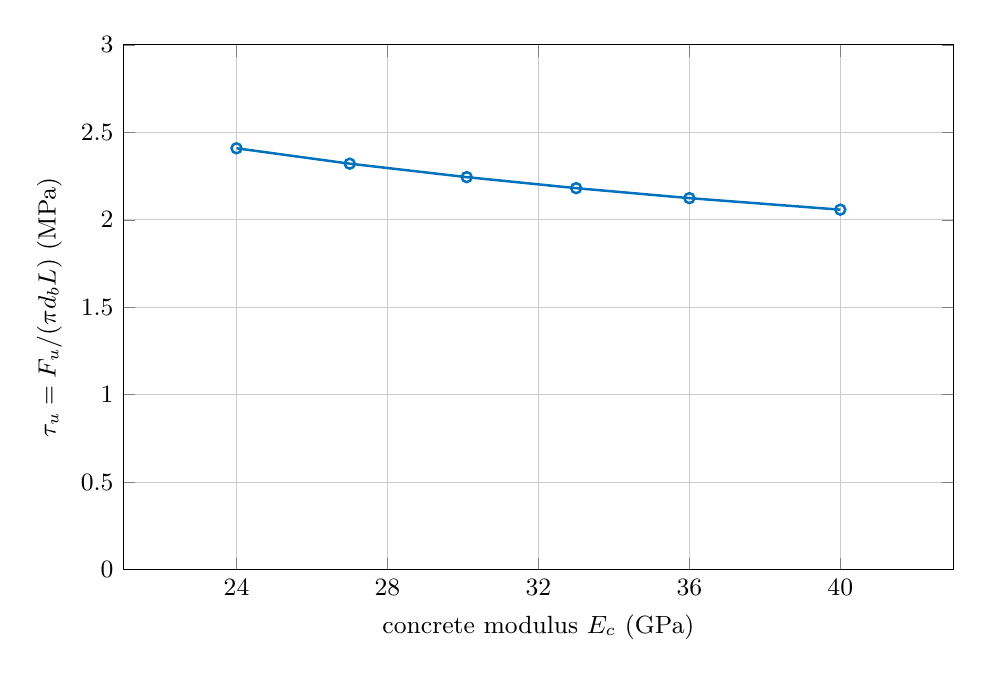
\begin{tikzpicture}
\begin{axis}[ecaxis,
  ylabel={$\tau_u = F_u/(\pi d_b L)$ (MPa)},
  ymin=0, ymax=3, ytick={0,0.5,1,1.5,2,2.5,3}]
\addplot[mblue] coordinates {
  (24.0,2.409) (27.0,2.321) (30.1,2.244)
  (33.0,2.181) (36.0,2.124) (40.0,2.058)};
\end{axis}
\end{tikzpicture}
\caption{}
\label{fig:factorEc-tau}
\end{subfigure}
\caption{Effect of concrete modulus at constant strength
         ($f'_c = \SI{32}{\mega\pascal}$, $d_b = \SI{12}{\milli\metre}$,
         $L = \SI{150}{\milli\metre}$, $r_e = \SI{75}{\milli\metre}$):
         (a)~cracking load, (b)~mean bond stress. Both \emph{fall} as the
         concrete stiffens, because $f_t$ and $f_v$ are held constant and
         only the stress distribution changes.}
\label{fig:factorEc}
\end{figure}
% ----------------------------------------------------------------------
\subsection{Tensile-to-shear strength ratio}
\label{sec:matratio}
 
Throughout this work the tensile and shear strengths have been set equal.
That equality is an assumption rather than a measurement, and because the
two enter the interaction index separately,
\begin{equation}
\label{eq:indexrecall}
\Phi_{II} = \left(\frac{\bar\sigma_\theta}{f_t}\right)^2
          + \left(\frac{\bar\tau_{rz}}{f_v}\right)^2 - 1 ,
\end{equation}
it must be established how much of the predicted capacity rests on it.
 
\begin{table}[H]
\centering
\caption{Effect of the shear-to-tensile strength ratio
         ($f_t = \SI{2.83}{\mega\pascal}$ held).}
\label{tab:sweepratio}
\small
\begin{tabular*}{\linewidth}{@{\extracolsep{\fill}}cccccc@{}}
\hline
$f_v/f_t$ & $f_v$ (MPa) & $F_{II}$ (kN) & $\tau_u$ (MPa)
          & $\hat\sigma$ & $\hat\tau$ \\
\hline
0.50 & 1.41 & 7.480  & 1.323 & 0.361 & 0.933 \\
0.75 & 2.12 & 10.406 & 1.840 & 0.502 & 0.865 \\
1.00 & 2.83 & 12.688 & 2.244 & 0.612 & 0.791 \\
1.25 & 3.54 & 14.415 & 2.549 & 0.695 & 0.719 \\
1.50 & 4.24 & 15.709 & 2.778 & 0.757 & 0.653 \\
2.00 & 5.66 & 17.418 & 3.080 & 0.840 & 0.543 \\
\hline
\end{tabular*}
\end{table}
 
The dependence is strong near the baseline: halving the assumed shear
strength cuts the predicted capacity by \SI{41}{\percent} and doubling it
raises the capacity by \SI{37}{\percent}. This is the largest material
effect in the chapter.
 
It is not, however, a simple scaling, and the last two columns show why.
At the baseline ratio the shear term carries \SI{63}{\percent} of the
criterion against the hoop term's \SI{37}{\percent}, so failure is
shear-controlled and the model responds strongly to $f_v$. As $f_v$ rises
the shear term shrinks and hoop tension takes over above
$f_v/f_t \approx 1.30$, after which extra shear strength buys very little.
In the limit of an infinitely strong interface the capacity would reach
only \SI{20.7}{\kilo\newton}, \SI{63}{\percent} above the baseline,
because the concrete would split first. Appendix~\ref{app:exponents} gives
a closed form that reproduces every case in Table~\ref{tab:sweepratio} to
better than \SI{0.1}{\percent}; a fitted power law is accurate only to
\SI{6.5}{\percent} and should not be used outside the range tested.
 
The bond stiffness does not change at all across this sweep, as it should
not, because it comes from the elastic solution and the strengths do not
enter there.
 
Measuring $f_v$ for the concretes in the test database is therefore the
cheapest available improvement to the model, and should come before any
further calibration.

% ======================================================================
\subsection{Factors of minor influence}
\label{sec:matminor}
 
Three further factors were swept and are reported together because none of
them changes the answer appreciably. Table~\ref{tab:sweepminor} gives the
range covered in each case and the resulting sensitivities.
 
\begin{table}[H]
\centering
\caption{The three remaining factors, each swept over five values about
         the baseline. Changes are quoted across the range shown.}
\label{tab:sweepminor}
\small
\begin{tabular*}{\linewidth}{@{\extracolsep{\fill}}lcrrrr@{}}
\hline
Factor & range swept & $n(F_{II})$ & $n(k_s)$
       & $\Delta F_{II}$ & $\Delta k_s$ \\
\hline
Steel modulus $E_s$ (GPa) & 185--215   & $+0.309$ & $+0.615$
                          & \SI{+4.8}{\percent}  & \SI{+9.7}{\percent} \\
Poisson's ratio $\nu_c$   & 0.15--0.25 & $+0.022$ & $-0.043$
                          & \SI{+1.1}{\percent}  & \SI{-2.2}{\percent} \\
Rib modulus $E_r/E_c$     & 0.25--4.0  & $-0.008$ & $+0.013$
                          & \SI{-2.2}{\percent}  & \SI{+3.7}{\percent} \\
\hline
\end{tabular*}
\end{table}
 
\paragraph{A moderate exponent need not mean a moderate effect.}
The steel modulus carries an exponent of \num{0.309}, which by the
classification of Section~\ref{sec:factorsapproach} is moderate and
comparable to that of the concrete modulus. It nevertheless moves the
capacity by less than \SI{5}{\percent}, because $E_s$ is not a quantity
that varies: reinforcing steel is \SI{200}{\giga\pascal} to within a few
per cent whatever its grade, and the range swept here already spans more
variation than a designer would ever encounter. The exponent and the
percentage change are answering different questions, and this is the one
factor in the study where they point opposite ways.
 
\paragraph{Poisson's ratio and the rib modulus are negligible.}
Both exponents are below the \num{0.05} threshold. The rib modulus is the
stronger test of the two: changing it by a factor of sixteen, from a
quarter of the concrete modulus to four times it, moves the capacity by
\SI{2.2}{\percent}. Taken with the thickness result of
Section~\ref{sec:ribthick}, this establishes that neither property of the
rib layer is silently controlling the predictions, which matters because
the layer is an idealisation rather than a measured feature of the
specimen.

% ======================================================================
\newpage
\section{Synthesis}
\label{sec:paramsynth}
 
\subsection{Ranking the factors}
 
Table~\ref{tab:stiffsens} collects every sweep, ranked by the magnitude of
the capacity exponent, and sets the capacity and stiffness sensitivities
side by side.
 
\begin{table}[H]
\centering
\caption{Sensitivity of capacity and stiffness to every factor, ranked by
         $|n(F_{II})|$. Here $n$ is the exponent of a power law
         $F_{II} \propto x^{\,n}$ fitted across each swept range, as
         defined in Section~\ref{sec:factorsapproach}; the cover entries exclude
         the two clipped cases of Table~\ref{tab:sweepcover}.}
\label{tab:stiffsens}
\small
\begin{tabular*}{\linewidth}{@{\extracolsep{\fill}}lrrll@{}}
\hline
Factor & $n(F_{II})$ & $n(k_s)$ & class & direction \\
\hline
Bar diameter $d_b$           & $+0.886$ & $+1.318$ & dominant   & together \\
Strength ratio $f_v/f_t$\,$^{\dagger}$ & $+0.615$ & $0$ & dominant & capacity only \\
Concrete strength $f'_c$     & $+0.390$ & $+0.137$ & moderate   & together \\
Steel modulus $E_s$          & $+0.309$ & $+0.615$ & moderate   & together \\
Concrete modulus $E_c$       & $-0.308$ & $+0.384$ & moderate   & \emph{opposed} \\
Cover ratio $c/d_b$          & $+0.281$ & $-0.289$ & moderate   & \emph{opposed} \\
Embedment length $L$         & $+0.131$ & $+0.064$ & moderate   & together \\
Poisson's ratio $\nu_c$      & $+0.022$ & $-0.043$ & negligible & --- \\
Rib modulus $E_r/E_c$        & $-0.008$ & $+0.013$ & negligible & --- \\
Rib thickness $t_{rib}$      & $-0.001$ & $-0.001$ & negligible & --- \\
\hline
\end{tabular*}
\end{table}
 
\subsection{Capacity and stiffness are not governed alike}
 
Three patterns appear in Table~\ref{tab:stiffsens}.
 
Most factors move capacity and stiffness in the same direction, and for
those there is nothing further to say: a change that strengthens the
anchorage also stiffens it.
 
Two factors move them in \emph{opposite} directions. Raising the concrete
modulus stiffens the anchorage by \SI{22}{\percent} while reducing its
capacity by \SI{15}{\percent}; increasing the cover raises the capacity by
\SI{36}{\percent} while reducing the stiffness by \SI{28}{\percent}. Both
say the same thing differently: capacity is governed by the averaged stress
near the bar, whereas stiffness is governed by the compliance of the whole
load path, and a change that redistributes stress away from the bar surface
helps one and hurts the other. For design this means cover should not be
read as a single measure of anchorage quality. Extra cover improves
resistance to splitting, which is the role it plays in bond design, but it
does not improve behaviour at working load: on these results the anchorage
becomes slightly more flexible as cover grows, and the slip at first
cracking almost doubles across the range tested.
 
One factor moves capacity alone. The strength ratio $f_v/f_t$ enters only
the failure criterion and not the elastic solution, so it leaves $k_s$
exactly unchanged. This is useful for calibration: the stiffness provides a
check on the elastic model that is completely independent of the failure
criterion, so a model that predicts stiffness well but capacity poorly
localises the error to the criterion rather than to the stress field.
 
\subsection{Where the uncertainty sits}
 
Influence and uncertainty are not the same thing. Bar diameter is the most
influential factor in the study, but it is also known exactly for any real
anchorage, so however strongly it moves the capacity it adds nothing to the
uncertainty of a prediction. The strength ratio $f_v/f_t$ is the opposite
case. It is the next most influential factor, and it has never been
measured for the concretes in the test database, so its value is a choice
rather than a datum. Across the range swept here that choice alone moves
the predicted capacity by a factor of \num{2.3}.

Every other property in the study was measured: cover, concrete strength,
the three moduli, Poisson's ratio and the rib dimensions. Taken together
across their swept ranges they move the capacity by about a factor of two.
A single untested assumption therefore carries as much uncertainty as every
measured property of the specimen put together, which is the honest summary
of the model's present standing. Reducing that exposure is a matter of
measuring $f_v$ rather than assuming it.
 
% ======================================================================
\section{Conclusions}
\label{sec:paramconc}
 
The parametric study establishes the following.
 
\paragraph{Cracking capacity scales almost in proportion to bar
diameter.}
Both diameter sweeps return $F_{II} \propto d_b^{0.89}$ with
$R^2 > 0.999$, agreeing to within \SI{1.4}{\percent} although one holds the
embedment fixed and the other the slenderness. Since the force required to
yield a bar grows as $d_b^2$, anchoring large bars is disproportionately
harder, which is the mechanical basis of the constraint identified by
\textcite{ngChangesAustralianStandards} and investigated experimentally by
\textcite{fosterDevelopmentLapLengths}.
 
\paragraph{Cracking capacity and stiffness both level off within about
ten diameters.}
Capacity is flat beyond $L = \SI{100}{\milli\metre}$ for the baseline bar
and stiffness beyond \SI{125}{\milli\metre}, roughly eight and ten
diameters. Because the stiffness is computed from the elastic solution
alone, the levelling off is a property of the load transfer and not an
artefact of the failure criterion. The consequences for development length
are pursued in Chapter~\ref{chap:devlength}.
 
\paragraph{The concrete-strength exponent decomposes exactly.}
The measured $\tau_u \propto (f'_c)^{0.390}$ resolves into a strength
contribution of \num{0.500} and a modulus contribution of
$-0.308 \times 0.356 = -0.110$, reproducing the combined value to within
\num{0.0001}. This gives a mechanical explanation for why the empirical
exponent of \textcite{SpliceStrengthConventional2000} lies below the square
root, complementing the length-dependent explanation of
\textcite{harajliComparisonBondStrength2004}.
 
\paragraph{The predicted failure mode shifts with geometry.}
The index moves from shear-controlled to hoop-controlled as the bar diameter
passes about \SI{17}{\milli\metre}, and shifts the same way as cover
increases. This reproduces a pull-out to splitting transition the model was
not fitted to.
 
\paragraph{The model is robust to its invented parameters but not to one
assumption.}
An eightfold change in rib layer thickness moves the capacity by
\SI{0.15}{\percent} and a sixteenfold change in its modulus by
\SI{2.2}{\percent} (Sections~\ref{sec:ribthick} and~\ref{sec:matminor}), so
the three-layer idealisation is not silently controlling the results. The
exception is the assumption $f_v = f_t$: capacity changes by
\SI{133}{\percent} across a fourfold change in the assumed ratio, and the
baseline failure is shear-controlled. Measuring $f_v$ is the cheapest
available improvement to the model.
 
\paragraph{Cover is understated by construction.}
The averaging disc has a radius of \SI{26.4}{\milli\metre}, so concrete
beyond that distance is never sampled directly and reaches the criterion
only by stiffening the surrounding ring. The exponent of \num{0.281} should
therefore be read as a lower bound. The same radius produced the two
clipped cases of Table~\ref{tab:sweepcover}; repairing the response would
need a criterion that recognises the free surface, which is beyond the
present scope.
 
\paragraph{What follows.}
The capacities established here depend on four quantities a designer knows,
namely bar diameter, embedment length, cover and concrete strength, and on
two that must be calibrated, the critical distance $l_{char}$ and the
strength ratio $f_v/f_t$. Chapter~\ref{chap:devlength} assembles the first
four into a family of calibration curves, shows that the family collapses
onto a single master curve, and inverts that curve to give a development
length expression in which the bar grade appears exactly once.